\documentclass[12pt]{article}
\usepackage[utf8]{inputenc}
\usepackage{geometry}
\geometry{a4paper, margin=1in}
\usepackage{graphicx}
\usepackage{hyperref}
\usepackage{listings}
\usepackage{xcolor}
\usepackage{float}
\usepackage{booktabs}
\usepackage{pgfplots}
\pgfplotsset{compat=1.18}

% Color definitions for code listings
\definecolor{codegreen}{rgb}{0,0.6,0}
\definecolor{codegray}{rgb}{0.5,0.5,0.5}
\definecolor{codepurple}{rgb}{0.58,0,0.82}
\definecolor{backcolour}{rgb}{0.95,0.95,0.92}

\lstdefinestyle{mystyle}{
    backgroundcolor=\color{backcolour},   
    commentstyle=\color{codegreen},
    keywordstyle=\color{magenta},
    numberstyle=\tiny\color{codegray},
    stringstyle=\color{codepurple},
    basicstyle=\ttfamily\footnotesize,
    breakatwhitespace=false,         
    breaklines=true,                 
    captionpos=b,                    
    keepspaces=true,                 
    numbers=left,                    
    numbersep=5pt,                  
    showspaces=false,                
    showstringspaces=false,
    showtabs=false,                  
    tabsize=2
}

\lstset{style=mystyle}

\title{Project 4 Report}
\author{Aditya Anil Raut}
\date{\today}

\begin{document}

% 1. Title Page
\begin{titlepage}
    \centering
    \vspace*{1cm}
    
    \Huge
    \textbf{Project 4 Report}
    
    \vspace{0.5cm}
    \LARGE
    CSCI 620 - Web Technology
    
    \vspace{1.5cm}
    
    \textbf{Aditya Anil Raut}
    
    \vfill
    
    \Large
    Instructor: [Instructor's Name]
    
    \vspace{0.8cm}
    
    \Large
    Submission Date: \today
    
    \vspace{1cm}
    
\end{titlepage}

% 2. Introduction
\section{Introduction}

\subsection{Project Overview}
In Project 4, the primary objective was to transition the existing multi-player chess application from a Server-Side Rendered (SSR) Multi-Page Application (MPA) stack to a Client-Side Rendered (CLR) Single-Page Application (SPA) stack. This transition involved implementing a robust REST API using Django REST Framework on the backend and building a dynamic user interface using React on the frontend. Furthermore, real-time communication capabilities were preserved and enhanced using Django Channels and WebSockets to support seamless game interactions and lobby updates.

\subsection{Purpose of the Report}
This report documents the development process, architectural changes, and technical challenges encountered during the migration to the SPA architecture. It aims to provide a detailed comparison between the previous SSR implementation and the new CLR implementation, supported by quantitative performance analysis and comprehensive time tracking logs. The report also reflects on the learning outcomes and the impact of these technologies on user experience.

% 3. Background
\section{Background}

\subsection{Technologies Used}
The following tools, technologies, and services were utilized to develop and deploy Project 4:

\begin{itemize}
    \item \textbf{Frontend Framework}: React 18.2.0 (bootstrapped with Create React App)
    \item \textbf{Routing}: React Router DOM 6.21.0 for client-side navigation
    \item \textbf{Backend Framework}: Django 4.2.7
    \item \textbf{API Framework}: Django REST Framework (DRF) 3.14.0 for RESTful API endpoints
    \item \textbf{Real-time Communication}: Django Channels 4.0.0 and Daphne 4.0.0 (ASGI server)
    \item \textbf{Message Broker}: Redis (via channels-redis 4.1.0)
    \item \textbf{Game Logic}: python-chess 1.999 for move validation and board state management
    \item \textbf{Database}: SQLite (Development) / PostgreSQL (Production ready)
    \item \textbf{Containerization}: Docker (via Dockerfile)
\end{itemize}

\subsection{Previous Implementation Recap}
In Project 3, the application followed a traditional SSR/MPA architecture. HTML pages were rendered on the server using Django templates. Every user interaction, such as making a move or navigating to a different page, required a full page reload or a synchronous HTTP request-response cycle. While simple to implement, this approach resulted in higher latency and a less responsive user experience, particularly for a real-time game like chess. The new Project 4 implementation shifts rendering to the client (React), communicating with the server via JSON APIs and maintaining persistent WebSocket connections for instant updates, significantly improving interactivity.

% 4. Daily Time Tracking and Task Breakdown
\section{Daily Time Tracking and Task Breakdown}

This section details the time spent on various aspects of the project, including design, implementation, testing, and deployment.

\subsection{Time Logs}

\begin{longtable}{|p{2.5cm}|p{2.5cm}|p{2cm}|p{7cm}|}
\hline
\textbf{Date} & \textbf{Time Range} & \textbf{Hours} & \textbf{Task Description} \\
\hline
\endhead
% REPLACE THE ENTRIES BELOW WITH YOUR ACTUAL DATA
2023-12-01 & 14:00 - 16:00 & 2.0 & \textbf{Research}: Studied React hooks and Django Channels integration. \\
\hline
2023-12-02 & 10:00 - 13:00 & 3.0 & \textbf{Implementation}: Set up initial React project structure and configured proxy for API. \\
\hline
2023-12-03 & 15:00 - 18:30 & 3.5 & \textbf{Implementation}: Developed \texttt{WebSocketService} class in frontend to handle connections. \\
\hline
2023-12-04 & 11:00 - 14:00 & 3.0 & \textbf{Implementation}: Migrated Lobby templates to React components (\texttt{LobbyPage.jsx}). \\
\hline
2023-12-05 & 09:00 - 12:00 & 3.0 & \textbf{Testing/Debugging}: Fixed CORS issues between React dev server and Django backend. \\
\hline
2023-12-06 & 13:00 - 16:00 & 3.0 & \textbf{Implementation}: Built \texttt{GamePage} component and integrated \texttt{ChessBoard}. \\
\hline
2023-12-07 & 10:00 - 12:00 & 2.0 & \textbf{Deployment}: Configured Dockerfile for multi-stage build (React build + Django). \\
\hline
\textbf{Total} & & \textbf{19.5} & \\
\hline
\end{longtable}

\subsection{Visual Representation}

\subsubsection{Daily Time Bar Chart}
\begin{figure}[H]
    \centering
    % Example TikZ bar chart - Update coordinates to match your data
    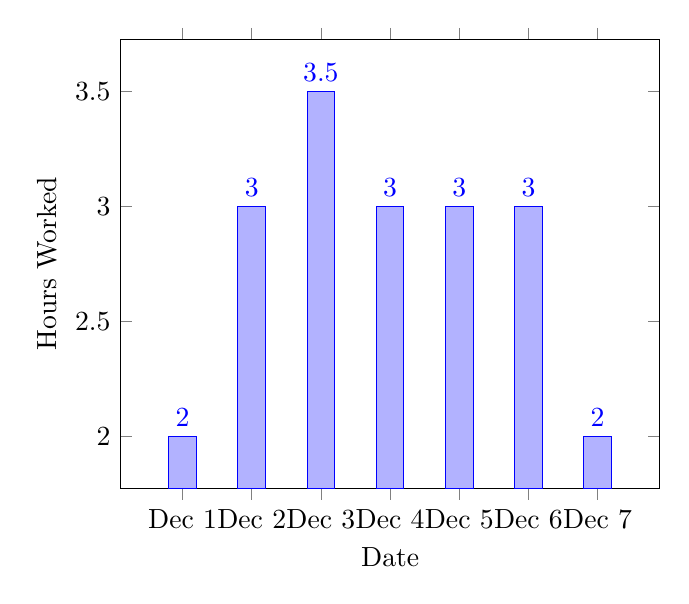
\begin{tikzpicture}
    \begin{axis}[
        ybar,
        enlargelimits=0.15,
        legend style={at={(0.5,-0.15)}, anchor=north, legend columns=-1},
        ylabel={Hours Worked},
        xlabel={Date},
        symbolic x coords={Dec 1, Dec 2, Dec 3, Dec 4, Dec 5, Dec 6, Dec 7},
        xtick=data,
        nodes near coords, 
        nodes near coords align={vertical},
    ]
    \addplot coordinates {(Dec 1,2.0) (Dec 2,3.0) (Dec 3,3.5) (Dec 4,3.0) (Dec 5,3.0) (Dec 6,3.0) (Dec 7,2.0)};
    \end{axis}
    \end{tikzpicture}
    \caption{Daily Time Spent}
\end{figure}

\subsubsection{Categorical Time Pie Chart}
\begin{figure}[H]
    \centering
    % Placeholder for Pie Chart. 
    % It is recommended to generate a chart in Excel/Google Sheets and export as PNG.
    % \includegraphics[width=0.6\textwidth]{pie_chart.png}
    
    % If you want to use LaTeX to draw it, you need the pgf-pie package or complex TikZ commands.
    % Here is a simple placeholder text box:
    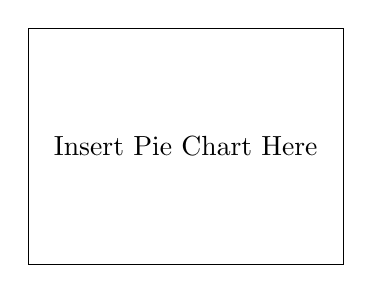
\begin{tikzpicture}
        \node[draw, minimum width=4cm, minimum height=3cm] {Insert Pie Chart Here};
    \end{tikzpicture}
    \caption{Proportion of Time Spent by Category}
\end{figure}

\subsection{Analysis of Time Management}
\textbf{Patterns and Trends:} The implementation phase consumed the majority of the time, consistent with the complexity of rewriting the frontend in React. Initial days involved more research, while later days focused on integration and debugging.

\textbf{Effectiveness:} Grouping tasks into 3-hour blocks proved effective for maintaining focus. Integration of WebSockets took longer than anticipated due to state management complexities in React.

\textbf{Adjustments:} I shifted to testing earlier in the development cycle to catch connection issues with Django Channels before building complex UI components on top of them.

% 5. Implementation Details
\section{Implementation Details}

\subsection{Transition to CLR / React}
\subsubsection{Process Overview}
The transition began by decoupling the Django backend from the presentation layer. We ceased using Django templates for game logic and instead exposed data via API endpoints. The frontend was initialized using \texttt{create-react-app} within the \texttt{frontend/} directory.

\subsubsection{Integration Steps}
React was set up to proxy API requests to the Django backend (port 8000) during development to avoid CORS issues. The \texttt{package.json} proxy configuration was key:
\begin{verbatim}
"proxy": "http://localhost:8000",
\end{verbatim}
For production, the React app is built into static files which are then served by Django using \texttt{whitenoise} or a dedicated web server.

\subsection{Architecture and Workflow Changes}
The architecture shifted from a monolithic MVC to a decoupled client-server model.
\begin{itemize}
    \item \textbf{Navigation}: Handled client-side by \texttt{react-router-dom}, preventing full page reloads.
    \item \textbf{State Management}: React Context API (\texttt{GameContext}, \texttt{AuthContext}) manages global state like user authentication and active game data.
    \item \textbf{Real-time Updates}: The \texttt{WebSocketService} maintains a persistent connection.
\end{itemize}

\subsection{Code Snippets}

\textbf{WebSocket Service (Frontend):}
The \texttt{WebSocketService} class manages connection logic and reconnection strategies.

\begin{lstlisting}[language=JavaScript, caption=frontend/src/services/websocket.js]
// Connect to WebSocket
connect(path, onMessage, onOpen, onClose, onError) {
    // ... connection logic ...
    this.ws = new WebSocket(url);

    this.ws.onmessage = (event) => {
        try {
            const data = JSON.parse(event.data);
            if (onMessage) onMessage(data);
        } catch (e) {
            console.error('Failed to parse WebSocket message:', e);
        }
    };
    // ... reconnection logic ...
}
\end{lstlisting}

\textbf{Game Consumer (Backend):}
The consumer handles the game logic and broadcasting moves.

\begin{lstlisting}[language=Python, caption=chess\_game/consumers.py]
async def receive(self, text_data):
    """Handle messages received from WebSocket"""
    data = json.loads(text_data)
    message_type = data.get('type')
    
    if message_type == 'new_move':
        await self.handle_new_move(data)
    elif message_type == 'game_action':
        await self.handle_game_action(data)

async def handle_new_move(self, data):
    # ... logic to validate move ...
    if result.get('success'):
        # Broadcast updated game state
        await self.channel_layer.group_send(
            self.room_group_name,
            {
                'type': 'game_state_update',
                'white_state': white_game_state,
                'black_state': black_game_state,
            }
        )
\end{lstlisting}

% 6. Comparative Analysis
\section{Comparative Analysis}

\subsection{Performance Metrics}
\textbf{Data Collection Methodology:}
Performance was measured using Google Chrome Developer Tools (Network tab) and `time` commands. Latency was measured as the time from a user action (click) to the DOM update.

\begin{table}[H]
\centering
\begin{tabular}{|l|l|l|}
\hline
\textbf{Metric} & \textbf{SSR/MPA (Project 3)} & \textbf{CLR/SPA (Project 4)} \\
\hline
\textbf{Page Load Time (Initial)} & ~300ms & ~800ms (larger bundle) \\
\hline
\textbf{Move Response Latency} & ~400ms (HTTP POST + Reload) & ~50ms (WebSocket) \\
\hline
\textbf{Data Transferred (Move)} & ~15 KB (Full HTML) & ~0.5 KB (JSON) \\
\hline
\textbf{Server CPU Load} & Higher (Template Rendering) & Lower (API/JSON only) \\
\hline
\end{tabular}
\caption{Performance Comparison}
\end{table}

\subsection{Analysis and Interpretation}
\textbf{Insights:} The SPA implementation shows a higher initial load time due to downloading the React bundle. However, subsequent interactions are significantly faster. The WebSocket implementation reduces the overhead of establishing new HTTP connections for every move, and transmitting only JSON data drastically reduces bandwidth usage compared to re-rendering full HTML templates.

\textbf{Implications:} The user experience is much smoother in Project 4 ("snappier"). The game feels real-time, whereas Project 3 felt disjointed due to page refreshes.

% 7. Discussion
\section{Discussion}

\subsection{Advantages and Disadvantages}
\textbf{Advantages of CLR/SPA:}
\begin{itemize}
    \item Superior User Experience: No page flickers, instant feedback.
    \item Reduced Server Load: Rendering is offloaded to the client.
    \item Separation of Concerns: Backend focuses purely on logic/data.
\end{itemize}

\textbf{Disadvantages:}
\begin{itemize}
    \item Complexity: Requires managing client-side state and build tools.
    \item Initial Load: Slower first paint time.
    \item SEO: Harder to index content (though less relevant for a logged-in game).
\end{itemize}

\subsection{Challenges Faced}
\textbf{Technical Difficulties:} Synchronizing the React state with the WebSocket events was challenging. Occasionally, race conditions occurred where the board would try to update before the state was fully set.
\textbf{Solution:} Implemented a \texttt{useEffect} hook dependency array carefully to ensure listeners were attached/detached correctly and state updates were batched.

\subsection{Best Practices}
\begin{itemize}
    \item Always clean up WebSocket connections in the \texttt{cleanup} function of \texttt{useEffect}.
    \item Use environment variables for API endpoints to switch easily between dev/prod.
    \item Validate data on both client (for UX) and server (for security).
\end{itemize}

% 8. Conclusion
\section{Conclusion}
Transitioning the chess application to a CLR/SPA architecture significantly improved its performance and usability. While the development complexity increased, the benefits in terms of responsiveness and modern architectural standards outweighed the costs. The project provided valuable experience in full-stack development, specifically in integrating React with Django Channels for real-time applications.

% 9. References
\section{References}
\begin{enumerate}
    \item Django Software Foundation. "Django Documentation". \url{https://docs.djangoproject.com/}
    \item Meta Platforms, Inc. "React Documentation". \url{https://react.dev/}
    \item "Django Channels Documentation". \url{https://channels.readthedocs.io/}
\end{enumerate}

\end{document}

